\chapter{Daten-Kompression}
In diesem Kapitel untersuchen wir die Frage, wie wir einen gegebenen String $s$ m\"oglichst platzsparend
abspeichern k\"onnen.  Wir gehen davon aus, dass der String $s$ aus Buchstaben besteht, die 
Elemente einer Menge $\Sigma$ sind.  Die Menge $\Sigma$ bezeichnen wir als unser \emph{Alphabet}. 
Wenn das Alphabet aus $n$ verschiedenen Zeichen besteht und wir alle Buchstaben mit derselben L\"ange
von $b$ Bits kodieren wollen, dann muss f\"ur diese Zahl von Bits offenbar
\[ n \leq 2^b \] 
gelten, woraus
\[ b = \textsl{ceil}\bigl(\log_2(n)\bigr) \]
folgt.  Hier bezeichnet $\textsl{ceil}(x)$ die \emph{Ceiling-Funktion}.  Diese Funktion
rundet eine gegebene reelle Zahl immer auf, es gilt also
\[ \textsl{ceil}(x) = \min \{ k \in \N \mid x \leq k \}. \]
Besteht der String $s$ aus $m$ Buchstaben, so werden zur Kodierung des Strings insgesamt
$m \cdot b$ Bits gebraucht.  Lassen wir die Forderung, dass alle Buchstaben mit derselben
Anzahl von Bits kodiert werden, fallen, dann ist es unter Umst\"anden m\"oglich, den String
$s$ mit weniger Bits zu kodieren.  Die zentrale Idee ist dabei, dass Buchstaben, die sehr
h\"aufig auftreten, mit m\"oglichst wenig Bits kodiert werden, w\"ahrend Buchstaben, die sehr selten
auftreten, mit einer gr\"o{\ss}eren Anzahl Bits kodiert werden.  Zur Verdeutlichung betrachten
wir folgendes Beispiel:  Unser Alphabet  $\Sigma$ bestehe nur aus vier Buchstaben,
\[ \Sigma = \{ \mathtt{a}, \mathtt{b}, \mathtt{c}, \texttt{d} \}. \]
In dem zu speichernden String $s$ trete der Buchstabe \texttt{a} insgesamt $990$ mal auf, der
Buchstabe \texttt{b} trete $8$ mal auf und die Buchstaben \texttt{c} und \texttt{d} treten
jeweil $1$ mal auf.  Dann besteht der String $s$ aus insgesamt $1\,000$ 
Buchstaben.  Wenn wir jeden Buchstaben mit $2 = \log_2(4)$ Bits kodieren, dann werden also
insgesamt $2\,000$ Bits ben\"otigt um den String $s$ abzuspeichern.  Wir k\"onnen den String
aber auch mit weniger Bits abspeichern, wenn wir die einzelnen Buchstaben mit Bitfolgen
unterschiedlicher L\"ange kodieren.   In unserem konkreten
Beispiel wollen wir versuchen den Buchstaben \texttt{a}, der mit Abstand am h\"aufigsten
vorkommt, mit einem einzigen Bit zu kodieren.  Bei den  Buchstaben
\texttt{c} und \texttt{d}, die nur sehr selten auftreten, ist es kein Problem auch mehr
Bits zu verwenden.  Tabelle \ref{tab:coding} zeigt eine Kodierung, die von dieser Idee
ausgeht. 

\begin{table}[htbp]
  \centering
\begin{tabular}[t]{|l|r|r|r|r|}
\hline
Buchstabe & \texttt{a} & \texttt{b}  & \texttt{c}   & \texttt{d}   \\
\hline
Kodierung & \texttt{0} & \texttt{10} & \texttt{110} & \texttt{111} \\
\hline
\end{tabular}
  \caption{Kodierung der Buchstaben mit variabler L\"ange.}
  \label{tab:coding}
\end{table}

Um zu verstehen, wie diese Kodierung funktioniert, stellen wir sie in
Abbildung \ref{fig:coding-tree} als Baum dar.  Die inneren 
Knoten dieses Baums enthalten keine Attribute und werden als leere Kreise dargestellt.
Die Bl\"atter des Baums sind mit den Buchstaben markiert.
Die Kodierung eines Buchstabens ergibt sich \"uber die Beschriftung der Kanten, die von dem
Wurzel-Knoten zu dem Buchstaben f\"uhren.  Beispielsweise f\"uhrt von der Wurzel eine
Kante direkt zu dem Blatt, das mit dem Buchstaben ``\texttt{a}'' markiert ist.  Diese
Kante ist mit dem Label ``\texttt{0}'' beschriftet.  Also wird der Buchstabe
``\texttt{a}'' durch den String ``\texttt{0}'' kodiert.  Um ein weiteres Beispiel zu
geben, betrachten wir den Buchstaben ``\texttt{c}''.   Der Pfad, der von der Wurzel zu dem
Blatt f\"uhrt, das mit ``\texttt{c}'' markiert ist, enth\"alt drei Kanten.  Die ersten beiden
Kanten sind jeweils mit ``\texttt{1}'' markiert, die letzte Kante ist mit ``\texttt{0}''
markiert.  Also wird der Buchstabe ''\texttt{c}'' durch den String ``\texttt{110}''
kodiert.  Kodieren wir nun unseren urspr\"unglichen String $s$, der aus $990$
\texttt{a}'s, $8$ \texttt{b}'s, einem \texttt{c} und einem \texttt{d} besteht, so
ben\"otigen wir insgesamt
\[ 990 \cdot 1 + 8 \cdot 2 + 1 \cdot 3 + 1 \cdot 3 = 1\,012 \]
Bits.  Gegen\"uber der urspr\"unglichen Kodierung, die $2\,000$ Bits verwendet, haben wir $49,4\%$
gespart!

\begin{figure}[!ht]
  \centering
  \framebox{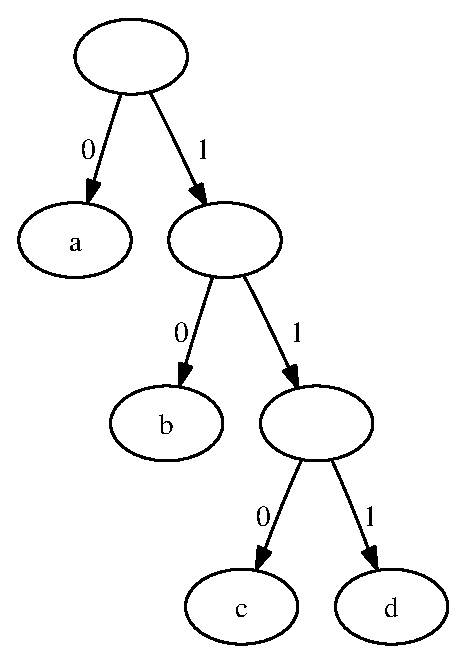
\epsfig{file=coding-tree.eps, scale=0.5}} 
  \caption{Baum-Darstellung der Kodierung.}
  \label{fig:coding-tree}
\end{figure}

Um zu sehen, wie mit Hilfe des Kodierungs-Baums ein String dekodiert werden kann,
betrachten wir als Beispiel den String ``\texttt{100111}''.  Wir beginnen mit der
``\texttt{1}'', die uns sagt, vom Wurzel-Knoten dem rechten Pfeil zu folgen.  Die
anschlie{\ss}ende ``\texttt{0}'' spezifiziert dann den linken Pfeil.  Jetzt sind wir bei dem
mit ''\texttt{b}'' markierten Blatt angekommen und haben damit den ersten Buchstaben
gefunden.  Wir gehen wieder zur Wurzel des Baums zur\"uck. Die folgende ``\texttt{0}'' f\"uhrt
uns zu dem Blatt, das mit ``\texttt{a}'' markiert ist, also haben wir den zweiten
Buchstaben gefunden. Wir gehen wieder zur Wurzel zur\"uck.  Die Ziffern ``\texttt{111}''
f\"uhren uns nun zu dem Buchstaben ``\texttt{d}''.  Damit haben wir insgesamt
\\[0.2cm]
\hspace*{1.3cm}
``\texttt{100111}'' $\simeq$ ``\texttt{bad}''.


\section{Der Algorithmus von Huffman}
Angenommen, wir haben einen String $s$, der aus Buchstaben eines Alphabets $\Sigma$
aufgebaut ist.  Wie finden wir dann eine Kodierung f\"ur die einzelnen Buchstaben, die
mit m\"oglichst wenig Bits auskommt?  Der Algorithmus von Huffman gibt eine Antwort auf diese
Frage. Um diesen Algorithmus pr\"asentieren zu k\"onnen, definieren wir die Menge
$\mathcal{K}$ der \emph{Kodierungs-B\"aume} induktiv.  
\begin{enumerate}
\item $\textsl{leaf}(c,f) \in \mathcal{K} \quad \mbox{falls $c \in \Sigma$ und $f \in \N$}$.

      Ausdr\"ucke der Form $\textsl{leaf}(c,f)$ sind die Bl\"atter eines Kodierungs-Baums.
      Dabei ist $c$ ein Buchstabe aus unserem Alphabet $\Sigma$ und $f$ gibt die
      H\"aufigkeit an, mit der dieser Buchstabe in dem zu kodierenden String auftritt.

      Gegen\"uber Abbildung \ref{fig:coding-tree} kommen hier bei den Bl\"attern noch die
      H\"aufigkeiten hinzu.  Diese ben\"otigen wir, denn wir wollen ja sp\"ater Buchstaben,
      die sehr h\"aufig auftreten, mit m\"oglichst wenig Bits kodieren.  

\item $\textsl{node}(l,r) \in \mathcal{K} \quad 
       \mbox{falls $l \in\mathcal{K}$ und $r \in \mathcal{K}$.}$ 

      Ausdr\"ucke der Form $\textsl{node}(l,r)$ sind die inneren Knoten eines
      Kodierungs-Baums.  
\end{enumerate}
Als n\"achstes  definieren wir eine Funktion 
\[  \textsl{count} : \mathcal{K} \rightarrow \N, \]
welche die  Gesamt-H\"aufigkeiten aller in dem Baum auftretenden Buchstaben aufsummiert.
\begin{enumerate}
\item Die Definition der Funktion \textsl{count} ist f\"ur Bl\"atter trivial:
      \[ \textsl{leaf}(c,f).\textsl{count}() = f. \]
\item Die Gesamt-H\"aufigkeit des Knotens $\textsl{node}(l,r)$
      ergibt sich als Summe der Gesamt-H\"aufigkeiten von $l$ und $r$. Also gilt
      \[ \textsl{node}(l,r).\textsl{count}() = l.\textsl{count}() + r.\textsl{count}(). \]
\end{enumerate}
Weiter definieren wir auf Kodierungs-B\"aumen die Funktion
\[ \textsl{cost}: \mathcal{K} \rightarrow \N. \]
Die Funktion \textsl{cost} gibt an, wie viele Bits ben\"otigt werden, um mit dem gegebenen
Kodierungs-Baum eine String zu kodieren, wenn die H\"aufigkeiten, mit denen ein Buchstabe
verwendet wird, mit den H\"aufigkeiten \"ubereinstimmen, die an den Bl\"attern des Baums notiert
sind.  Die Definition dieser Funktion ist induktiv:
\begin{enumerate}
\item $\textsl{leaf}(c,f).\textsl{cost}() = 0$,

      denn solange nur ein einziger Buchstabe vorhanden ist, ist noch nichts zu kodieren.
\item $\textsl{node}(l,r).\textsl{cost}() = 
       l.\textsl{cost}() + r.\textsl{cost}() + l.\textsl{count}() + r.\textsl{count}()$.

      Wenn wir zwei Kodierungs-B\"aume $l$ und $r$ zu einem neuen Kodierungs-Baum
      zusammenf\"ugen, verl\"angern sich die Kodierungen f\"ur alle Buchstaben, die in $l$ oder
      $r$ auftreten, um ein Bit.
      Die Summe 
      \[ l.\textsl{count}() + r.\textsl{count}() \]
      gibt die Gesamt-H\"aufigkeiten aller Buchstaben an, die in dem linken und
      rechten Teilbaum auftreten.  Da sich die Kodierung aller dieser Buchstaben
      durch die Bildung des Knotens $\textsl{node}(l,r)$ gegen\"uber der Kodierung in $l$
      und $r$ jeweils um 1 verl\"angert, m\"ussen wir zu den Kosten der Teilb\"aume $l$ und $r$
      den Term $l.\textsl{count}() + r.\textsl{count}()$ hinzuaddieren.
\end{enumerate}
Wir erweitern die Funktion $\textsl{cost}()$ auf Mengen von Knoten, indem wir die Kosten
einer Menge $M$ als die Summe der Kosten der Knoten von $M$ definieren:
\[ \textsl{cost}(M) = \sum\limits_{n\in M} n.\textsl{cost}(). \]
Ausgangs-Punkt des von David A.~Huffman (1925 -- 1999) \cite{huffman:52} angegebenen
Algorithmus ist eine Menge von Paaren der Form $\langle c, f\rangle$.  Dabei ist $c$ ein
Buchstabe und $f$ gibt die H\"aufigkeit an, mit der dieser Buchstabe auftritt.  Im ersten
Schritt werden diese Paare in die Bl\"atter eines Kodierungs-Baums \"uberf\"uhrt.  Besteht der
zu kodierende String aus  $n$ verschiedenen Buchstaben, so haben
wir dann eine Menge von Kodierungs-B\"aumen der Form
\begin{equation}
  \label{eq:huffmann1}
 M = \bigl\{ \textsl{leaf}(c_1,f_1), \cdots, \textsl{leaf}(c_k,f_k) \bigr\}   
\end{equation}
Es werden nun solange Knoten $a$ und $b$ aus $M$ zu einem neuen Knoten
$\textsl{node}(a,b)$ zusammengefasst, bis die Menge $M$ nur noch einen Knoten enth\"alt.
Offenbar gibt es im Allgemeinen sehr viele M\"oglichkeiten, die Knoten aus der Menge zu
neuen Knoten zusammen zu fassen.  Das Ziel ist es die Knoten so zusammen zu fassen, dass
die Kosten der Menge $M$ am Ende  minimal sind.
Um zu verstehen, welche Knoten wir am geschicktesten zusammenfassen k\"onnen, betrachten wir, wie
sich die Kosten der Menge durch das Zusammenfassen zweier Knoten \"andert.
Dazu betrachten wir zwei Mengen von Knoten $M_1$ und $M_2$, so dass 
\[ M_1 = N \cup \{ a, b\} \quad \mathtt{und} \quad M_2 = N \cup \{ \textsl{node}(a,b) \} \]
gilt, die Menge $M_1$ geht also aus der Menge $M_2$ dadurch hervor, dass wir
die Knoten $a$ und $b$ zu einem neuen Knoten zusammen fassen und durch diesen ersetzen.
Untersuchen wir, wie
sich die Kosten der Menge dabei ver\"andern, wir untersuchen also die folgende Differenz:
\begin{eqnarray*}
& & \textsl{cost}\bigl(N \cup \{ \textsl{node}(a,b) \}\bigr) - \textsl{cost}\bigl(N \cup \{ a,b \}\bigr) \\
&=& \textsl{cost}\bigl( \{ \textsl{node}(a,b) \}\bigr) - \textsl{cost}\bigl(\{ a,b \}\bigr)              \\
&=& \textsl{node}(a,b).\textsl{cost}() - a.\textsl{cost}() - b.\textsl{cost}()                           \\
&=&   a.\textsl{cost}() + b.\textsl{cost}() + a.\textsl{count}() + b.\textsl{count}() 
    - a.\textsl{cost}() - b.\textsl{cost}()                                                              \\
&=& a.\textsl{count}() + b.\textsl{count}() 
\end{eqnarray*}
Fassen wir die Knoten $a$ und $b$ aus der Menge $M$ zu einem neuen Knoten zusammen, so verg\"o{\ss}ern sich
die Kosten der Menge um die Summe
\[ a.\textsl{count}() + b.\textsl{count}(). \]
Wenn wir die Kosten der Menge $M$ insgesamt m\"oglichst klein halten wollen, dann ist es daher naheliegend,
dass wir in der Menge $M$ die beiden Knoten $a$ und $b$ suchen, f\"ur die die Funktion
$\textsl{count}()$ den kleinsten Wert liefert.  Diese Knoten werden wir aus der Menge $M$
entfernen und durch den neuen Knoten $\textsl{node}(a,b)$ ersetzen.
Dieser Prozess wird solange iteriert, bis die Menge $M$ nur noch aus einem Knoten besteht.  Dieser
Knoten ist dann die Wurzel des gesuchten Kodierungs-Baums. 
Der in Abbildung \ref{fig:huffman} gezeigte Pseudo-Code beschreibt diesen Algorithmus.

\begin{figure}[!ht]
\centering
\begin{Verbatim}[ frame         = lines, 
                  framesep      = 0.3cm, 
                  labelposition = bottomline,
                  numbers       = left,
                  numbersep     = -0.2cm,
                  xleftmargin   = 1.3cm,
                  xrightmargin  = 1.3cm,
                  codes         = {\catcode`_=8\catcode`$=3},
                  commandchars  = \\\{\},
                ]
    procedure codingTree(M) \{
        while (#M > 1) \{
            a := minCount(M);
            M := M - \{ a \};
            b := minCount(M);
            M := M - \{ b \};
            M := M + \{ node(a, b) \};
        \}
        return arb M;
    \}
\end{Verbatim}
\vspace*{-0.3cm}
\caption{Der Algorithmus von Huffman.}
\label{fig:huffman}
\end{figure} % $

\begin{enumerate}
\item Die Funktion \textsl{codingTree} wird mit einer Menge $M$ von Knoten aufgerufen,
      welche die in Gleichung (\ref{eq:huffmann1}) angegebene Form hat.
\item Die \texttt{while}-Schleife veringert die Anzahl der Knoten in der Menge $M$
      in jedem Schritt um Eins.  
      \begin{enumerate}
      \item Dazu werden mit Hilfe der Funktion $\textsl{minCount}()$ die
            beiden Knoten $a$ und $b$ berechnet, f\"ur die der Wert von $\textsl{count}()$ minimal
            ist.  Beide Knoten werden aus der Menge $M$ entfernt.

            Die Funktion $\textsl{minCount}(M)$ berechnet den Knoten der Menge $M$, f\"ur den 
            die Funktion $\textsl{count}()$ den kleinsten Wert annimmt, es gilt also
            \[ \textsl{minCount}(M) = m \;\rightarrow\; 
               \forall n \in M: m.\textsl{count}() \leq n.\textsl{count}() \]
      \item Anschlie{\ss}end wird aus den beiden Knoten $a$ und $b$ ein neuer Knoten 
            $\textsl{node}(a,b)$ gebildet.
            Dieser Knoten wird der Menge $M$ hinzugef\"ugt.
      \end{enumerate}
\item Die \texttt{while}-Schleife wird beendet, wenn die Menge $M$ nur noch ein Element enth\"alt.
      Dieses wird mit der Funktion \texttt{arb} extrahiert und als Ergebnis zur\"uck gegeben.
\end{enumerate}
Die Laufzeit des Huffman-Algorithmus h\"angt stark von der Effizienz der Funktion $\textsl{minCount}()$.
Eine naive Implementierung w\"urde die Knoten aus der Menge $M$ in einer geordneten Liste vorhalten.
Die Knoten $n$ w\"aren in dieser Liste nach der Gr\"o{\ss}e $n.\textsl{cost}()$ aufsteigend sortiert.
Dann ist die Funktion $\textsl{minCount}()$ zwar sehr effizient, aber die Operation
\\[0.2cm]
\hspace*{1.3cm}
\texttt{M := M + \{ node(a, b) \};}
\\[0.2cm]
w\"urde einen Aufwand erfordern, der linear in der Anzahl der Elemente der Menge $M$ ist.
Es ist effizienter, die Menge $M$ durch eine Priorit\"ats-Warteschlange $Q$ darzustellen, denn
dann kann die Funktion $\textsl{minCount}()$ durch $Q.\textsl{top}()$ realisiert werden, w\"ahrend
das Einf\"ugen von $\textsl{Node}(a,b)$ durch den Aufruf von $\textsl{insert}()$ realisiert wird.

\begin{table}[htbp]
  \centering
\begin{tabular}[t]{|l|r|r|r|r|r|}
\hline
Buchstabe  & \texttt{a} & \texttt{b} & \texttt{c} & \texttt{d} & \texttt{e} \\
\hline
H\"aufigkeit &          1 &          2 &          3 &          4 &          5 \\
\hline
\end{tabular}
  \caption{Buchstaben mit H\"aufigkeiten.}
  \label{tab:frequency}
\end{table}

Wir illustrieren den  Huffman-Algorithmus, indem wir ihn auf die Buchstaben, die in
Tabelle \ref{tab:frequency} zusammen mit ihren H\"aufigkeiten angegeben sind, anwenden.
\begin{enumerate}
\item Zu Beginn hat die Menge $M$ die Form
      \\[0.2cm]
      \hspace*{0.3cm}
      $ M = \bigl\{ \textsl{leaf}(\mathtt{a},1),\,
             \textsl{leaf}(\mathtt{b},2),\, 
             \textsl{leaf}(\mathtt{c},3),\,
             \textsl{leaf}(\mathtt{d},4),\,
             \textsl{leaf}(\mathtt{e},5)\bigr\}. $
\item Die Funktion $\textsl{count}()$ ist hier f\"ur die Bl\"atter mit den Buchstaben \texttt{a} und
      \texttt{b} minimal.  Also entfernen wir diese Bl\"atter aus der Menge und f\"ugen statt
      dessen den Knoten 
      \\[0.2cm]
      \hspace*{0.3cm}
      $\textsl{node}\bigl(\textsl{leaf}(\mathtt{a},1), \textsl{leaf}(\mathtt{b},2)\bigr)$
      \\[0.2cm]
      in die Menge $M$ ein.  Es gilt
      \\[0.2cm]
      \hspace*{0.3cm}
      $\textsl{node}\bigl(\textsl{leaf}(\mathtt{a},1), \textsl{leaf}(\mathtt{b},2)\bigr).\textsl{count}()
       = \textsl{leaf}(\mathtt{a},1).\textsl{count}()+  \textsl{leaf}(\mathtt{b},2).\textsl{count}()
       = 1 + 2 = 3$.
      \\[0.2cm]
      Um die Funktion $\textsl{count}()$ nicht jedes Mal neu berechnen zu m\"ussen, annotieren wir
      den Wert dieser Funktion mit einem Doppelpunkt an einem Knoten $n$ in der Form 
      \\[0.2cm]
      \hspace*{0.3cm}
      $n:n.\textsl{count}()$.
      \\[0.2cm]
      Dann hat $M$ die Form
      \\[0.2cm]
      \hspace*{0.3cm}
      $ \bigl\{\textsl{node}\bigl(\textsl{leaf}(\mathtt{a},1), \textsl{leaf}(\mathtt{b},2)\bigr):3,\,
             \textsl{leaf}(\mathtt{c},3),\, \textsl{leaf}(\mathtt{d},4),\,
             \textsl{leaf}(\mathtt{e},5)\bigr\}. $
\item Die beiden Knoten mit den kleinsten Werten von \textsl{count} sind nun
      \\[0.2cm]
      \hspace*{0.3cm}
      $ \textsl{node}(\textsl{leaf}(\mathtt{a},1), \textsl{leaf}(\mathtt{b},2)):3 
         \quad \mathrm{und} \quad \textsl{leaf}(\mathtt{c},3). $
      \\[0.2cm]
      Wir entfernen diese beiden Knoten und bilden aus den beiden Knoten den neuen Knoten
      \\[0.2cm]
      \hspace*{0.3cm}
      $ \textsl{node}\Bigl(
           \textsl{node}\bigl((\textsl{leaf}(\mathtt{a},1), \textsl{leaf}(\mathtt{b},2)\bigr),\; 
           \textsl{leaf}(\mathtt{c},3)\Bigr):6, $
      \\[0.2cm]
      den wir der Menge $M$ hinzuf\"ugen.  Dann hat $M$ die Form
      \\[0.2cm]
      \hspace*{0.3cm}
      $ \Bigl\{ 
        \textsl{leaf}(\mathtt{d},4),\;\textsl{leaf}(\mathtt{e},5),\;
        \textsl{node}\Bigl(
           \textsl{node}\bigl(\textsl{leaf}(\mathtt{a},1), \textsl{leaf}(\mathtt{b},2)\bigr),\; 
           \textsl{leaf}(\mathtt{c},3)\Bigr):6\Bigr\}. $
\item Jetzt sind 
      \\[0.2cm]
      \hspace*{0.3cm}
      $ \textsl{leaf}(\mathtt{d},4) \quad \mathrm{und} \quad \textsl{leaf}(\mathtt{e},5)$
      \\[0.2cm]
      die beiden Knoten mit dem kleinsten Werten von \textsl{count}.
      Wir entfernen diese Knoten und bilden den neuen Knoten \\[0.2cm]
      \hspace*{0.3cm}
      $ \textsl{node}\bigl(\textsl{leaf}(\mathtt{d},4), \textsl{leaf}(\mathtt{e},5)\bigr):9. $
      \\[0.2cm]
      Diesen f\"ugen wir der Menge $M$ hinzu und erhalten
      \\[0.2cm]
      \hspace*{0.3cm}
      $ \Bigl\{ 
        \textsl{node}\bigl(\textsl{leaf}(\mathtt{d},4), \textsl{leaf}(\mathtt{e},5)\bigr):9,\;
        \textsl{node}\Bigl(
           \textsl{node}\bigl(\textsl{leaf}(\mathtt{a},1), \textsl{leaf}(\mathtt{b},2)\bigr),\; 
           \textsl{leaf}(\mathtt{c},3)\Bigr):6\Bigr\}. $      
\item Jetzt enth\"alt die Menge $M$ nur noch zwei Knoten.  Wir entfernen diese Knoten und
      bilden daraus den neuen Knoten
      \\[0.2cm]
      \hspace*{0.3cm}
      $\textsl{node}\Bigl(
              \textsl{node}\Bigl(
                 \textsl{node}\bigl(\textsl{leaf}(\mathtt{a},1), \textsl{leaf}(\mathtt{b},2)\bigr),\; 
                 \textsl{leaf}(\mathtt{c},3)\Bigr),\;
              \textsl{node}\bigl(\textsl{leaf}(\mathtt{d},4), \textsl{leaf}(\mathtt{e},5)\bigr)
         \Bigr):15
      $
      \\[0.2cm]
      Dieser Knoten ist jetzt der einzige Knoten in $M$ und damit unser Ergebnis.
      Stellen wir diesen Knoten als Baum dar, so erhalten wir das in Abbildung
      \ref{fig:coding-tree2} gezeigte Ergebnis.  Wir haben hier jeden Knoten $n$
      mit dem Funktionswert  $n.\textsl{count}()$ beschriftet.  

      Die Kodierung, die sich daraus ergibt,
      wird in Tabelle \ref{tab:coding2} gezeigt.
\end{enumerate}

\begin{figure}[!ht]
  \centering
  \framebox{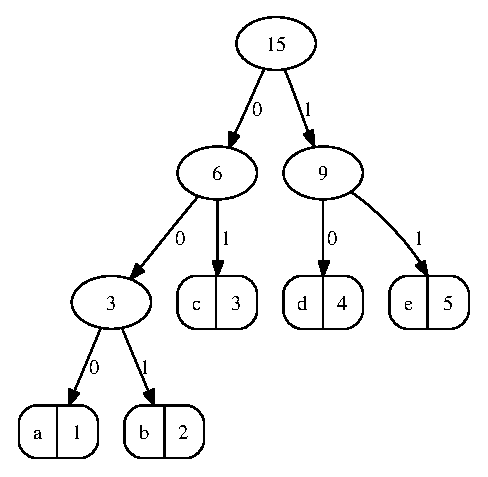
\epsfig{file=coding-tree2.eps, scale=0.7}} 
  \caption{Baum-Darstellung der Kodierung.}
  \label{fig:coding-tree2}
\end{figure}



\begin{table}[htbp]
  \centering
\begin{tabular}[t]{|l|r|r|r|r|r|}
\hline
Buchstabe &   \texttt{a} &   \texttt{b} & \texttt{c}  & \texttt{d}  & \texttt{e}   \\
\hline
Kodierung & \texttt{000} & \texttt{001} & \texttt{01} & \texttt{10} & \texttt{11} \\
\hline
\end{tabular}
  \caption{Kodierung der Buchstaben mit variabler L\"ange.}
  \label{tab:coding2}
\end{table}


\subsection{Implementierung in \textsl{Java}}
\begin{figure}[!ht]
\centering
\begin{Verbatim}[ frame         = lines, 
                  framesep      = 0.3cm, 
                  labelposition = bottomline,
                  numbers       = left,
                  numbersep     = -0.2cm,
                  xleftmargin   = 0.8cm,
                  xrightmargin  = 0.8cm,
                ]
    public abstract class Node implements Comparable<Node> {
    	public    abstract Integer cost();
    	public    abstract Integer count();
    
    	public int compareTo(Node rhs) {
    		return count().compareTo(rhs.count());
    	}
    
    }
\end{Verbatim}
\vspace*{-0.3cm}
\caption{Die abstrakte Klasse \texttt{Node}.}
\label{fig:Huffman/Node.java}
\end{figure}

\noindent
Wir zeigen nun, wie die Berechnung des Huffman-Codes in \textsl{Java} implementiert werden
kann.  Als erstes pr\"asentieren wir Klassen, um Kodierungs-B\"aume darstellen zu
k\"onnen.  Abbildung \ref{fig:Huffman/Node.java} zeigt die Implementierung der abstrakten
Klasse \texttt{Node}, mit der wir Elemente der Menge der Kodierungs-B\"aume $\mathcal{K}$ darstellen.
Da wir sp\"ater Knoten anhand der f\"ur diesen Knoten  gespeicherten H\"aufigkeiten vergleichen
m\"ussen, implementiert diese Klasse die Schnittstelle \texttt{Comparable}.
Dazu muss die Klasse \texttt{Node} die Methode $\textsl{compareTo}()$ bereitstellen.  
Diese Methode vergleicht verschiedene Knoten \"uber die Werte der Funktion $\textsl{count}()$.

\begin{figure}[!ht]
\centering
\begin{Verbatim}[ frame         = lines, 
                  framesep      = 0.3cm, 
                  labelposition = bottomline,
                  numbers       = left,
                  numbersep     = -0.2cm,
                  xleftmargin   = 0.8cm,
                  xrightmargin  = 0.8cm,
                ]
    public class LeafNode extends Node {
        private char mCharacter;
        private int  mFrequency;
        
        public LeafNode(char character, int frequency) {
            mCharacter = character;
            mFrequency = frequency;
        }
        public Integer cost() {
            return 0;
        }
        public Integer count() {
            return mFrequency;
        }
        public Character getCharacter() {
            return mCharacter;
        }
    }
\end{Verbatim}
\vspace*{-0.3cm}
\caption{Die Klasse \texttt{Leaf}.}
\label{fig:Leaf.java}
\end{figure}

Die Klasse \texttt{LeafNode} repr\"asentiert Knoten der Form $\textsl{leaf}(c,f)$.
Der Buchstabe $c$ wird in der Member-Variablen \texttt{mCharacter} abgespeichert und die H\"aufigkeit
$f$, mit der dieser Buchstabe in dem zu kodierenden String $s$ auftritt, wird in der
Member-Variablen \texttt{mFrequency} abgelegt.
\begin{enumerate}
\item Der Konstruktor initialisiert die beiden Member-Variablen \texttt{mCharacter} und
      \texttt{mFrequency}. 
\item Die Funktion $\textsl{cost}()$ liefert als Ergebnis $0$, denn f\"ur Bl\"atter hatten wir 
      \\[0.2cm]
      \hspace*{1.3cm}
      $\textsl{leaf}(c,f).\textsl{cost}() = 0$
      \\[0.2cm]
      definiert.
\item Die Funktion $\textsl{count}()$ liefert die H\"aufigkeit \texttt{mFrequency}, denn f\"ur Bl\"atter hatten wir
      \\[0.2cm]
      \hspace*{1.3cm}
      $\textsl{leaf}(c,f).\textsl{count}() = f$
      \\[0.2cm]
      definiert.
\item Die Funktion $\textsl{getCharacter}()$ gibt als Ergebnis den in der Member-Variablen \texttt{mCharacter}
      gespeicherten Buchstaben zur\"uck.
\end{enumerate}

\begin{figure}[!ht]
\centering
\begin{Verbatim}[ frame         = lines, 
                  framesep      = 0.3cm, 
                  labelposition = bottomline,
                  numbers       = left,
                  numbersep     = -0.2cm,
                  xleftmargin   = 0.8cm,
                  xrightmargin  = 0.8cm,
                ]
    public class BinaryNode extends Node {
        private Node mLeft;
        private Node mRight;
        private int  mCount;
        private int  mCost;
    
        public BinaryNode(Node left, Node right) {
            mLeft  = left;
            mRight = right;
            mCount = mLeft.count() + mRight.count();
            mCost  = mLeft.cost()  + mRight.cost() + mCount;
        }
        public Integer cost() {
            return mCost;
        }
        public Integer count() {
            return mCount;
        }
    }
\end{Verbatim}
\vspace*{-0.3cm}
\caption{Die Klasse BinaryNode.}
\label{fig:Huffman/BinaryNode.java}
\end{figure}

Die Klasse \texttt{BinaryNode} repr\"asentiert einen bin\"aren Knoten der Form
$\textsl{node}(l,r)$.  Die Klasse hat vier Member-Variablen:
\begin{enumerate}
\item \texttt{mLeft}  speichert den linken  Teilbaum $l$ des Knotens $\textsl{node}(l,r)$.
\item \texttt{mRight} speichert den rechten Teilbaum $r$ des Knotens $\textsl{node}(l,r)$.
\item \texttt{mCount} speichert den Wert der Funktion $\textsl{node}(l,r).\textsl{count}()$.
      Wir speichern diesen Wert in einer Member-Variablen, damit wir ihn nur einmal berechnen
      m\"ussen.
\item \texttt{mCost}  speichert den Wert der Funktion $\textsl{node}(l,r).\textsl{cost}()$.
\end{enumerate}
Der Konstruktor der Klasse \texttt{BinaryNode} bekommt als Argumente den linken Teilbaum $l$ und den
rechten Teilbaum $r$ des zu konstruierenden Knotens $\textsl{node}(l,r)$.  Au{\ss}erdem berechnet der
Konstruktor die Werte $\textsl{node}(l,r).\textsl{count}()$ und $\textsl{node}(l,r).\textsl{cost}()$
und speichert diese Werte in den Member-Variablen \texttt{mCount} und \texttt{mCost}.


\begin{figure}[!h]
\centering
\begin{Verbatim}[ frame         = lines, 
                  framesep      = 0.3cm, 
                  labelposition = bottomline,
                  numbers       = left,
                  numbersep     = -0.2cm,
                  xleftmargin   = 0.3cm,
                  xrightmargin  = 0.3cm,
                ]
    import java.util.*;
    import java.io.*;
    
    public class Huffman {
        Map<Character, Integer> mFrequencyTable;
        Node                    mCoding;      // the coding tree 
    
        public Huffman(String fileName) {
            determineFrequencies(fileName);
            mCoding = createHuffmanCode();
        }
        public void determineFrequencies(String fileName) {
            mFrequencyTable = new TreeMap<Character, Integer>();
            for (char c = 1; c < 128; ++c) {
                mFrequencyTable.put(c, 0);
            }
            try {
                FileReader fr = new FileReader(fileName);
                while (true) {
                    char c = (char) fr.read();
                    if (c == 65535) { break; }
                    int count = mFrequencyTable.get(c);
                    ++count;
                    mFrequencyTable.put(c, count);
                }
            } catch (IOException e) {
                e.printStackTrace();
            }
        }    
        public Node createHuffmanCode() {
            PriorityQueue<Node> queue = new PriorityQueue<Node>();
            for (Character c: mFrequencyTable.keySet()) {
                Integer frequency = mFrequencyTable.get(c);
                if (frequency >= 1) {
                    LeafNode leaf = new LeafNode(c, frequency);
                    queue.offer(leaf);
                }
            }
            while (queue.size() > 1) {
                Node left  = queue.remove();
                Node right = queue.remove();
                Node node  = new BinaryNode(left, right);
                queue.offer(node);
            }
            return queue.peek();
        }
    }
\end{Verbatim}
\vspace*{-0.3cm}
\caption{Die Klasse Huffman.}
\label{fig:Huffman.java}
\end{figure}

Die Abbildung \ref{fig:Huffman.java} auf Seite \pageref{fig:Huffman.java} zeigt die
Implementierung der Klasse \texttt{Huffman}, die f\"ur einen gegebenen String den
Huffman-Code berechnet. 
Die Klasse \texttt{Huffman} enth\"alt zwei Member-Variablen:
\begin{enumerate}
\item \texttt{mFrequencyTable} ist eine Abbildung, die f\"ur jeden Buchstaben $c$, der in
      der gegebenen Datei auftritt, angibt, wie oft dieser Buchstabe in der Datei auftritt.
\item \texttt{mCoding} ist ein Knoten der Form $\textsl{node}(l,r)$.  Dieser Knoten ist
      das Endergebnis der Berechnung und enth\"alt den Kodierungs-Baum f\"ur den
      gegebenen Text.
\end{enumerate}
Wir besprechen jetzt die Details der Implementierung des Konstruktors und der Methoden in der Klasse
Huffman.
\begin{enumerate}
\item Der Konstruktor der Klasse \texttt{Huffman} bekommt als Argument den Namen der Datei, die
      den Text enth\"alt, f\"ur den der Huffman-Code bestimmt werden soll.  Anschlie{\ss}end liest
      die Methode $\textsl{determineFrequencies}()$  die angegebene Datei und berechnet die H\"aufigkeiten,
      mit denen die einzelnen Buchstaben auftreten.  Diese H\"aufigkeiten dann werden in der
      Tabelle \texttt{mFrequencyTable} abgespeichert.  Daraus berechnet die Methode
      $\textsl{createHuffmanCode}()$ den Huffman-Code mit Hilfe dieser Tabelle.
\item Die Methode $\textsl{determineFrequencies}()$ geht davon aus, dass als Zeichen nur
      Buchstaben aus dem \textsc{Ascii}-Zeichensatz verwendet werden.
      \begin{enumerate}
      \item Zun\"achst wird daher eine Tabelle f\"ur die 127 Zeichen aus dem
            \textsc{Ascii}-Zeichensatz angelegt.   Diese Tabelle soll jedem 
            Buchstaben die H\"aufigkeit, mit der dieser Buchstabe in der Datei auftritt,
            zuordnen.  Die Eintr\"age dieser Tabelle werden 
            in der \texttt{for}-Schleife in Zeile 15 zun\"achst mit 0 initialisiert.
            Sp\"ater wird jedesmal,  wenn wir einen Buchstaben lesen, die dem Buchstaben
            zugeordnete H\"aufigkeit inkrementiert.
      \item Anschlie{\ss}end wir die Datei in Zeile 18 zum Lesen ge\"offnet.
      \item In der anschlie{\ss}enden \texttt{while}-Schleife wird die Datei zeichenweise
            gelesen.  Falls dabei das Datei-Ende-Zeichen \texttt{EOF} gelesen wird,
            bricht diese Schleife durch den \texttt{break}-Befehl in Zeile 21 ab. 
            
            Wurde ein Zeichen $c$ gelesen, so wird zun\"achst in der Tabelle
            \texttt{mFrequencyTable} nachgeschlagen, wie h\"aufig dieses Zeichen schon
            aufgetreten ist.  Diese Zahl wird um 1 inkrementiert und die inkrementierte
            Zahl wird wieder in die Tabelle zur\"uckgeschrieben.
            
            Da die IO-Operationen in Zeile 18 und Zeile 20 Ausnahmen ausl\"osen k\"onnen,
            m\"ussen diese Anweisungen in einem \texttt{try}-\texttt{catch}-Block eingerahmt
            werden.
      \end{enumerate}
\item Die Methode $\textsl{createHuffmanCode}()$ implementiert den Algorithmus von Huffman.
      \begin{enumerate}
      \item Zun\"achst wird in Zeile 31 eine neue Priorit\"ats-Warteschlange angelegt.
      \item In der \texttt{for}-Schleife in Zeile 32 iterieren wir \"uber alle Zeichen.
            Falls ein Zeichen mindestens einmal in dem Text vorkommt,
            erzeugen wir in Zeile 35 einen Knoten $\textsl{leaf}(c,f)$ und f\"ugen diesen
            Knoten der Priorit\"ats-Warteschlange hinzu.
      \item Die \texttt{while}-Schleife in Zeile 39 implementiert den Pseudo-Code aus 
            Abbildung \ref{fig:huffman}:  Wir entfernen die beiden Knoten $l$ und $r$ mit den
            niedrigsten Priorit\"aten aus der Priorit\"ats-Warteschlange und bilden den neuen
            Knoten $\textsl{node}(l,r)$, den wir statt dessen in die
            Priorit\"ats-Warteschlange einf\"ugen.  Wenn die Priorit\"ats-Warteschlange nur noch
            genau einen Knoten enth\"alt, sind wir am Ziel und geben diesen Knoten 
            als Ergebnis zur\"uck.
      \end{enumerate}
\end{enumerate}

\noindent
\textbf{Aufgabe}:
\begin{enumerate}
\item Berechnen Sie den Huffman-Code f\"ur einen Text, der nur die Buchstaben
      ``\texttt{a}'' bis ``\texttt{g}'' enth\"alt und f\"ur den die H\"aufigkeiten,
      mit denen diese Buchstaben auftreten, durch die folgende Tabelle gegeben sind.

\begin{table}[htbp]
  \centering
\begin{tabular}[t]{|l|r|r|r|r|r|r|r|}
\hline
Buchstabe  & \texttt{a} & \texttt{b} & \texttt{c} & \texttt{d} & \texttt{e} & \texttt{f} & \texttt{g} \\
\hline
H\"aufigkeit &          1 &          1 &          2 &          3 &          5 &         8 &         13 \\
\hline
\end{tabular}
  \caption{Buchstaben mit H\"aufigkeiten.}
  \label{tab:aufgabe-huffman}
\end{table}

\item Wie gro{\ss} ist die Einsparung, wenn man die Buchstaben mit einem Huffman-Code
      kodiert gegen\"uber einer Kodierung mit drei Bits?
\item Versuchen Sie das Gesetz zu erkennen, nach dem die H\"aufigkeiten in der obigen Tabelle 
      gebildet wurden und versuchen Sie, den Huffman-Code f\"ur den allgemeinen Fall,
      in dem $n$ Buchstaben gegeben sind, anzugeben.
\item Wie gro{\ss} ist die Einsparung im allgemeinen Fall?
\end{enumerate}

\section{Optimalit\"at des Huffman'schen Kodierungsbaums}
In diesem Abschnitt zeigen wir, dass der durch den Algorithmus von Huffman berechnete Kodie\-rungs-Baum der
Kodierungs-Baum ist, f\"ur den die Funktion $\textsl{cost}()$ minimal ist.  Dazu geben zun\"achst eine andere
Formel zur Berechnung von $n.\textsl{cost}()$ an:  Wir definieren die \emph{Tiefe}
$n.\textsl{depth}(c)$ des Buchstabens $c$ in dem Kodierungs-Baum $n$ als den Abstand, den das Blatt $l$,
das mit dem Buchstaben $c$ markiert ist, von der Wurzel des Kodierungs-Baums hat.  Der Kodierungs-Baum
wird dabei als Graph aufgefasst.  Dann gibt es genau einen Pfad von der Wurzel zu dem Blatt $l$ und 
$n.\textsl{depth}(c)$ wird als die Anzahl der Kanten dieses Pfades definiert.
Jede der Kanten dieses Pfades tr\"agt hinterher ein Bit zur 
Kodierung des Buchstabens bei, mit dem das Blatt $l$ markiert ist.  Um die gesamten Kosten zu berechnen
m\"ussen wir daher die Tiefe jedes Buchstabens mit seiner H\"aufigkeit multiplizieren.  Bezeichnen wir die
H\"aufigkeit des Buchstabens $c$ mit $\textsl{freq}(c)$, so erhalten wir insgesamt
\begin{equation}
  \label{eq:cost}
  n.\textsl{cost}() = \sum\limits_{c\in\Sigma} \textsl{freq}(c) \cdot n.\textsl{depth}(c)
\end{equation}
Die Summe l\"auft dabei \"uber alle Buchstaben des Alphabets $\Sigma$, wobei wir voraussetzen,
dass alle Buchstaben aus $\Sigma$ auch tats\"achlich in dem Kodierungs-Baum auftreten.
Buchstaben, die gar nicht auftreten, werden also vorher aus dem Alphabet entfernt.

\begin{Definition}[Optimaler Kodierungs-Baum]
  Ein Kodierungs-Baum $n$ ist \emph{optimal}, wenn bei gegebener H\"aufigkeit der Buchstaben
  der Wert $n.\textsl{cost}()$ minimal ist, f\"ur alle Kodierungs-B\"aume $k$, bei denen die
  Buchstaben mit derselben H\"aufigkeit auftreten wie in $n$,  gilt also
  \\[0.2cm]
  \hspace*{1.3cm} $n.\textsl{cost}() \leq k.\textsl{cost}()$.
\end{Definition}


\begin{Lemma}
  \label{huffman:l1}
  Es seien $x$ und $y$ die beiden Buchstaben aus dem Alphabet $\Sigma$ mit der geringsten H\"aufigkeit.  Dann
  gibt es einen optimalen Kodierungs-Baum $n$, bei dem sich die Kodierung der Buchstaben $x$ und $y$ nur im
  letzten Bit unterscheidet.
\end{Lemma}

\noindent
\textbf{Beweis}:  Es sei $n_1$ ein optimaler Kodierungs-Baum.  Wir zeigen, wie $n_1$ zu einem
Kodierungs-Baum $n_2$ umgebaut werden kann, der einerseits optimal ist und bei dem sich andererseits die
Kodierung der Buchstaben $x$ und $y$ nur im letzten Bit unterscheidet.  Wir suchen in dem Kodierungs-Baum
$n_1$ einen Knoten $k$ der Form $\textsl{node}(l,r)$, der unter allen \emph{inneren} Knoten eine maximale
Tiefe hat.  Dabei bezeichnen wir alle Knoten, die keine Bl\"atter sind, als innere Knoten.
An dem Knoten $k$ h\"angen zwei Buchstaben $a$ und $b$.  Wir machen nun o.B.d.A.~die folgenden Annahmen
\"uber die H\"aufigkeiten der Buchstaben:
\begin{enumerate}
\item $\textsl{freq}(x) \leq \textsl{freq}(y)$,
\item $\textsl{freq}(a) \leq \textsl{freq}(b)$.
\end{enumerate}
Da wir angenommen haben, dass $x$ und $y$ die Buchstaben mit der geringsten H\"aufigkeiten sind, folgt
daraus
\begin{equation}
  \label{eq:huffmannL0}
\textsl{freq}(x) \leq \textsl{freq}(a) \quad \textrm{und} \quad 
\textsl{freq}(y) \leq \textsl{freq}(b).  
\end{equation}
Wir erhalten nun den Kodierungs-Baum $n_2$ aus dem Kodierungs-Baum $n_1$, indem wir in dem Baum $n_1$ die
Positionen der Buchstaben $x$ und $a$ und die Positionen der Buchstaben $y$ und $b$ vertauschen.
Daher gilt 
  \begin{eqnarray}
    \label{eq:huffmannL1a}
 n_2.\textsl{depth}(a) &=& n_1.\textsl{depth}(x), \\
    \label{eq:huffmannL1b}
 n_2.\textsl{depth}(b) &=& n_1.\textsl{depth}(y), \\
    \label{eq:huffmannL1c}
 n_2.\textsl{depth}(x) &=& n_1.\textsl{depth}(a), \\
    \label{eq:huffmannL1d}
 n_2.\textsl{depth}(y) &=& n_1.\textsl{depth}(b).
  \end{eqnarray}
denn $a$ und $x$ und $b$ und $y$ vertauschen die Pl\"atze.  F\"ur alle Buchstaben
$c \in \Sigma\backslash\{a,b,x,y\}$ gilt nat\"urlich 
\begin{equation}
  \label{eq:huffmannL1e}
n_2.\textsl{depth}(c) = n_1.\textsl{depth}(c).   
\end{equation}
Weiterhin wissen wir aufgrund der Auswahl des Knotens $k$, dass
\begin{eqnarray}
  \label{eq:huffmannL2a}
  n_1.\textsl{depth}(a) = n_1.\textsl{depth}(b) \geq n_1.\textsl{depth}(x) \quad \mathrm{und} \\
  \label{eq:huffmannL2b}
  n_1.\textsl{depth}(a) = n_1.\textsl{depth}(b) \geq n_1.\textsl{depth}(y) \hspace*{0.95cm}
\end{eqnarray}
gilt.  Wir zeigen nun, dass $n_2.\textsl{cost}() \leq n_1.\textsl{cost}()$ gilt.  Dazu geben wir zun\"achst
$n_2.\textsl{cost}()$ an.
\begin{eqnarray*}
  n_2.\textsl{cost}() 
  & = & \sum\limits_{c\in\Sigma} \textsl{freq}(c) \cdot n_2.\textsl{depth}(c) \\
  & = & \sum\limits_{c\in\Sigma\backslash\{a,b,x,y\}} \textsl{freq}(c) \cdot n_2.\textsl{depth}(c) \\[0.3cm]
  &   & + \;\textsl{freq}(a) \cdot n_2.\textsl{depth}(a) 
        + \textsl{freq}(b) \cdot n_2.\textsl{depth}(b) \\[0.1cm]
  &   & + \;\textsl{freq}(x) \cdot n_2.\textsl{depth}(x) 
        + \textsl{freq}(y) \cdot n_2.\textsl{depth}(y) 
\end{eqnarray*}
Unter Ber\"ucksichtigung der Gleichungen (\ref{eq:huffmannL1a}) bis (\ref{eq:huffmannL1e}) k\"onnen wir dies
auch schreiben als
\begin{eqnarray*}  
  n_2.\textsl{cost}() 
  & = & \sum\limits_{c\in\Sigma\backslash\{a,b,x,y\}} \textsl{freq}(c) \cdot n_1.\textsl{depth}(c) \\[0.3cm]
  &   & + \;\textsl{freq}(a) \cdot n_1.\textsl{depth}(x) 
        + \textsl{freq}(b) \cdot n_1.\textsl{depth}(y) \\[0.1cm]
  &   & + \;\textsl{freq}(x) \cdot n_1.\textsl{depth}(a) 
        + \textsl{freq}(y) \cdot n_1.\textsl{depth}(b) 
\end{eqnarray*}
Analog berechnen wir $n_1.\textsl{cost}()$:
\begin{eqnarray*}
  n_1.\textsl{cost}() 
  & = & \sum\limits_{c\in\Sigma} \textsl{freq}(c) \cdot n_1.\textsl{depth}(c) \\
  & = & \sum\limits_{c\in\Sigma\backslash\{a,b,x,y\}} \textsl{freq}(c) \cdot n_1.\textsl{depth}(c) \\[0.3cm]
  &   & + \;\textsl{freq}(a) \cdot n_1.\textsl{depth}(a) 
        + \textsl{freq}(b) \cdot n_1.\textsl{depth}(b) \\[0.1cm]
  &   & + \;\textsl{freq}(x) \cdot n_1.\textsl{depth}(x) 
        + \textsl{freq}(y) \cdot n_1.\textsl{depth}(y) 
\end{eqnarray*}
Damit sehen wir, dass $n_2.\textsl{cost}() \leq n_1.\textsl{cost}()$ genau dann gilt, wenn die
Ungleichung 
\\[0.2cm]
\hspace*{0.8cm}
$\textsl{freq}(a) \cdot n_1.\textsl{depth}(x) 
      + \textsl{freq}(b) \cdot n_1.\textsl{depth}(y) 
      + \textsl{freq}(x) \cdot n_1.\textsl{depth}(a) 
      + \textsl{freq}(y) \cdot n_1.\textsl{depth}(b)$ \\[0.1cm]
\hspace*{0.3cm}
$\leq\; \textsl{freq}(a) \cdot n_1.\textsl{depth}(a) 
      + \textsl{freq}(b) \cdot n_1.\textsl{depth}(b) 
      + \textsl{freq}(x) \cdot n_1.\textsl{depth}(x) 
      + \textsl{freq}(y) \cdot n_1.\textsl{depth}(y)$ \\[0.2cm]
erf\"ullt ist.  Da in dieser Ungleichung nur noch der Knoten $n_1$ vorkommt, vereinfachen wir die
Schreibweise und vereinbaren, dass wir einen Ausdruck der Form $n_1.\textsl{depth}(u)$ zu
$\textsl{depth}(u)$ abk\"urzen.  Die letzte Ungleichung ist dann \"aquivalent zu der Ungleichung
\\[0.2cm]
\hspace*{0.8cm}
$0 \;\leq\; \textsl{freq}(a) \cdot \bigl(\textsl{depth}(a) - \textsl{depth}(x)\bigr)
          + \textsl{freq}(b) \cdot \bigl(\textsl{depth}(b) - \textsl{depth}(y)\bigr)$ 
\\[0.2cm]
\hspace*{1.3cm}
$        -\;\textsl{freq}(x) \cdot \bigl(\textsl{depth}(a) - \textsl{depth}(x)\bigr) 
         - \textsl{freq}(y) \cdot \bigl(\textsl{depth}(b) - \textsl{depth}(y)\bigr)$ \\[0.2cm]
Diese Ungleichung vereinfachen wir zu 
\\[0.3cm]
\hspace*{0.3cm}
$0 \;\leq\; 
  \underbrace{\bigl(\textsl{freq}(a) - \textsl{freq}(x)\bigr)}_{\geq 0}   \cdot 
  \underbrace{\bigl(\textsl{depth}(a) - \textsl{depth}(x)\bigr)}_{\geq 0}
+ \underbrace{\bigl(\textsl{freq}(b) - \textsl{freq}(y)\bigr)}_{\geq 0}   \cdot 
  \underbrace{\bigl(\textsl{depth}(b) - \textsl{depth}(y)\bigr)}_{\geq 0}$
\\[0.3cm]
Hier gilt $\textsl{freq}(a) - \textsl{freq}(x) \geq 0$ wegen Ungleichung \ref{eq:huffmannL0},
die Ungleichung $\textsl{depth}(a) - \textsl{depth}(x) \geq 0$ folgt aus Ungleichung \ref{eq:huffmannL2a},
die Ungleichung $\textsl{freq}(b) - \textsl{freq}(y) \geq 0$ folgt aus Ungleichung \ref{eq:huffmannL0}
und die Ungleichung $\textsl{depth}(b) - \textsl{depth}(y) \geq 0$ 
folgt aus Ungleichung \ref{eq:huffmannL2b}.
Damit haben wir 
\[ n_2.\textsl{cost}() \leq n_1.\textsl{cost}() \]
gezeigt.  Da $n_1$ optimal ist, muss auch $n_2$ optimal sein.  Nach Wahl des Knotens $k$ unterscheiden
sich die Kodierungen von $x$ und $y$ nur in dem letzten Bit. Damit ist $n_2$ der gesuchte
Kodierungs-Baum.
\hspace*{\fill} $\Box$

\begin{Satz}
  Der Kodierungs-Baum, der von dem Huffman-Algorithmus erzeugt wird, ist optimal.
\end{Satz}

\noindent
\textbf{Beweis}:  Wir beweisen den Satz durch Induktion \"uber die Anzahl $n$ der Buchstaben in dem
Alphabet $\Sigma$.
\begin{enumerate}
\item[I.A.:] $n = 2$.  Es sei $\Sigma= \{a,b\}$.
  In diesem Fall f\"uhrt der Huffman-Algorithmus nur einen Schritt durch und liefert den Kodierungs-Baum 
  \\[0.2cm]
  \hspace*{1.3cm}
  $k=\textsl{node}\bigl(\textsl{leaf}(a, \textsl{freq}(a)), \textsl{leaf}(b,\textsl{freq}(b))\bigr)$.
  \\[0.2cm]
  Bei der Kodierung eines Alphabets, das aus zwei Buchstaben besteht, haben wir keine Wahl, 
  was die L\"ange der Kodes angeht: Wir brauchen f\"ur jeden Buchstaben genau ein Bit und daher ist das vom
  Huffman-Algorithmus in diesem Fall gelieferte Ergebnis offenbar optimal.
\item[I.S.:] $n \mapsto n+1$

  Wir gehen jetzt davon aus, dass das Alphabet $\Sigma$ aus $n+1$ Buchstaben besteht.
  Es seien $x$ und $y$ die beiden Buchstaben, deren H\"aufigkeit minimal ist.
  Es sei $z$ ein neuer Buchstabe, der nicht in dem Alphabet $\Sigma$ auftritt.  Wir definieren
  ein neues Alphabet $\Sigma'$ als
  \\[0.2cm]
  \hspace*{1.3cm}
  $\Sigma' = \bigl(\Sigma \backslash \{x,y\}\bigr) \cup \{z\}$.
  \\[0.2cm]
  Die H\"aufigkeit des neuen Buchstabens $z$ definieren wir als 
  \\[0.2cm]
  \hspace*{1.3cm}
  $\textsl{freq}(z) := \textsl{freq}(x) + \textsl{freq}(y)$.
  \\[0.2cm]
  Dann enth\"alt das Alphabet $\Sigma'$ insgesamt $n$ Buchstaben.  Wenden wir den Huffman-Algorithmus
  auf dieses Alphabet an, so erhalten wir nach Induktions-Voraussetzung f\"ur $\Sigma'$ einen optimalen
  Kodierungs-Baum $k_1$.  Die Anwendung des Huffman-Algorithmus auf das Alphabet $\Sigma$ ersetzt in diesem
  Kodierungs-Baum das Blatt, das mit dem Buchstaben $z$ markiert ist, durch den Knoten 
  \\[0.2cm]
  \hspace*{1.3cm}
  $\textsl{node}\bigl(\textsl{leaf}(x, \textsl{freq}(x)), \textsl{leaf}(y,\textsl{freq}(y))\bigr)$.
  \\[0.2cm]
  Bezeichnen wir den so entstanden Kodierungs-Baum mit $k_2$, so m\"ussen wir zeigen, dass $k_2$ optimal
  ist.  Wir f\"uhren den Beweis indirekt und nehmen an, dass $k_2$ nicht optimal ist. Dann gibt es einen
  Kodierungs-Baum $k_3$ f\"ur das Alphabet $\Sigma$, so dass 
  \\[0.2cm]
  \hspace*{1.3cm}
  $k_3.\textsl{cost}() < k_2.\textsl{cost}()$
  \\[0.2cm]
  ist.  Nach Lemma \ref{huffman:l1} k\"onnen wir o.B.d.A. voraussetzen, dass sich die Kodierung der 
  Buchstaben $x$ und $y$ in dem Kodierungs-Baum $k_3$ nur in dem letzten Bit
  unterscheidet.  Also gibt es in dem Kodierungs-Baum $k_3$ einen Knoten der Form
  \\[0.2cm]
  \hspace*{1.3cm}
  $\textsl{node}\bigl(\textsl{leaf}(x, \textsl{freq}(x)), \textsl{leaf}(y,\textsl{freq}(y))\bigr)$.
  \\[0.2cm]
  Wir transformieren den Kodierungs-Baum $k_3$ in einen Kodierungs-Baum $k_4$ f\"ur das Alphabet $\Sigma'$ indem
  wir diesen Knoten durch das Blatt
  \\[0.2cm]
  \hspace*{1.3cm}
  $\textsl{leaf}\bigl(z, \textsl{freq}(x) + \textsl{freq}(y)\bigr)$
  \\[0.2cm]
  ersetzen.  Damit gilt
  \begin{eqnarray*}
      k_4.\textsl{cost}() 
  &=& \sum\limits_{c\in\Sigma'} \textsl{freq}(c) \cdot k_4.\textsl{depth}(c) \\[0.3cm]
  &=& \sum\limits_{c\in\Sigma\backslash\{x,y\}\cup\{z\}} \textsl{freq}(c) \cdot k_4.\textsl{depth}(c) 
      \\[0.3cm]
  &=& \sum\limits_{c\in\Sigma\backslash\{x,y\}} \textsl{freq}(c) \cdot k_4.\textsl{depth}(c) 
      +\textsl{freq}(z) \cdot k_4.\textsl{depth}(z) \\[0.3cm]  
  &=& \sum\limits_{c\in\Sigma\backslash\{x,y\}} \textsl{freq}(c) \cdot k_3.\textsl{depth}(c) 
      +\textsl{freq}(z) \cdot \bigl(k_3.\textsl{depth}(x) - 1\bigr) \\[0.3cm]  
  &=& \sum\limits_{c\in\Sigma\backslash\{x,y\}} \textsl{freq}(c) \cdot k_3.\textsl{depth}(c) \\[0.3cm]
  & & +\; \bigl(\textsl{freq}(x) + \textsl{freq}(y)\bigr) \cdot \bigl(k_3.\textsl{depth}(x) - 1\bigr) 
      \\[0.3cm]  
  &=& \sum\limits_{c\in\Sigma} \textsl{freq}(c) \cdot k_3.\textsl{depth}(c) -\; \bigl(\textsl{freq}(x) + \textsl{freq}(y)\bigr)  
      \\[0.3cm]  
  &=& k_3.\textsl{cost}() - \bigl(\textsl{freq}(x) + \textsl{freq}(y)\bigr)  
  \end{eqnarray*}
  Wir halten dieses Ergebnis in einer Gleichung fest:
  \begin{equation}
    \label{eq:huffmanns1}
    k_4.\textsl{cost}() = k_3.\textsl{cost}() - \bigl(\textsl{freq}(x) + \textsl{freq}(y)\bigr).
  \end{equation}
  Da die Kodierungs-B\"aume $k_1$ und $k_2$ in derselben Relation stehen wie die Kodierungs-B\"aume
  $k_4$ und $k_3$, gilt analog
  \begin{equation}
    \label{eq:huffmanns2}
    k_1.\textsl{cost}() = k_2.\textsl{cost}() - \bigl(\textsl{freq}(x) + \textsl{freq}(y)\bigr). 
  \end{equation}
  Damit k\"onnen wir zeigen, dass die Kosten des Kodierungs-Baums $k_4$ geringer sind als die Kosten
  des Kodierungs-Baums $k_1$:
  \begin{eqnarray*}
         k_4.\textsl{cost}() 
   & = & k_3.\textsl{cost}() - \bigl(\textsl{freq}(x) + \textsl{freq}(y)\bigr) \\[0.1cm]
   & < & k_2.\textsl{cost}() - \bigl(\textsl{freq}(x) + \textsl{freq}(y)\bigr) \\[0.1cm] 
   & = & k_1.\textsl{cost}(). 
  \end{eqnarray*}
  Dieses Ergebnis steht aber im Widerspruch dazu, dass der Kodierungs-Baum $k_1$ 
  optimal ist.  Folglich ist die Annahme $k_3.\textsl{cost}() < k_2.\textsl{cost}()$ falsch und der
  Kodierungs-Baum $k_2$ ist bereits optimal.
  \hspace*{\fill} $\Box$
\end{enumerate}


%%% Local Variables: 
%%% mode: latex
%%% TeX-master: "algorithmen"
%%% End: 
